%\documentclass[overheadsbeamer.tex]{subfiles}
\documentclass[handoutsbeamer.tex]{subfiles}

\begin{document}

\thispagestyle{empty}

\ona{ \setcounter{chapter}{10} } % ONE LESS
\lecture{Warm-Started Quantum Optimization: Continuous}{Lect11}
\chapter{Warm-Started Quantum Optimization: Continuous}\label{C.WSContinuous}

\ona{This \chap{} continues \citet{egger2021warm}. Instead of rounding the relaxation classically and warm-starting from a cut (\Chap~\chref{C.WSRounded}), we warm-start from the \emph{continuous} solution of a convex relaxation and let the quantum measurement do the rounding. The mixer is modified so that the warm state is its ground state, which keeps the convergence guarantee of \Chap~\chref{C.QAOA}, and the regularisation $\varepsilon$ connects the method continuously to standard QAOA.}

\section{Warm-starting from a continuous relaxation}

\begin{frame}\ft{Continuous warm start}
\ona{In QAOA each binary variable $x_i$ corresponds to a qubit via $x_i = (1-z_i)/2$ and $z_i \mapsto Z_i$ gives $H_C$. The final measurement is a randomized rounding. The simplest warm start (WS-QAOA) replaces $\ket{+}^{\otimes n}$ by the product state encoding the \eqref{eq:ch10:qp} optimum $c^\star$,}
\begin{equation}\label{eq:ch11:init}
    \ket{\phi^\star} = \bigotimes_{i=1}^n R_Y(\theta_i)\ket{0}, \qquad \theta_i = 2\arcsin\sqrt{c_i^\star},
\end{equation}
\ona{so that qubit $i$ reads $1$ with probability $c_i^\star$ (Fig.~\ref{fig:ch11:bloch}), and replaces the mixer by}
\begin{align}\label{eq:ch11:mixer}
    H_M^{(\rm ws)} &= \sum_i H_{M,i}^{(\rm ws)},\\
    H_{M,i}^{(\rm ws)} &= \begin{pmatrix} 2c_i^\star - 1 & -2\sqrt{c_i^\star(1-c_i^\star)}\\ -2\sqrt{c_i^\star(1-c_i^\star)} & 1-2c_i^\star\end{pmatrix} = -\sin\theta_i\,X - \cos\theta_i\,Z,\nonumber
\end{align}
\ona{which has $R_Y(\theta_i)\ket0$ as ground state with eigenvalue $-1$, so $\ket{\phi^\star}$ is the ground state of $H_M^{(\rm ws)}$ with eigenvalue $-n$. The mixing gate $e^{-i\beta H_{M,i}^{(\rm ws)}}$ is a rotation about the axis $(-\sin\theta_i, 0, -\cos\theta_i)$ and compiles to $R_Y(\theta_i)R_Z(-2\beta)R_Y(-\theta_i)$, Fig.~\ref{fig:ch11:circuit}.}
\onp{Initial state: product state with $\Pr[x_i = 1] = c_i^\star$. Mixer: rotated so that $\ket{\phi^\star}$ is its ground state; compiles to $R_Y(\theta_i)R_Z(-2\beta)R_Y(-\theta_i)$.}
\end{frame}

\begin{frame}\ft{The warm initial state and circuit}
\onp{\begin{center}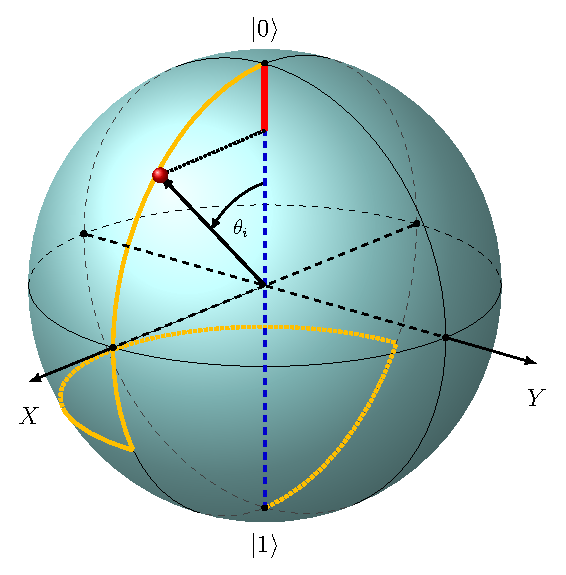
\includegraphics[height=0.45\textheight]{figures/warmstart/figure01.pdf}\hspace{0.5cm}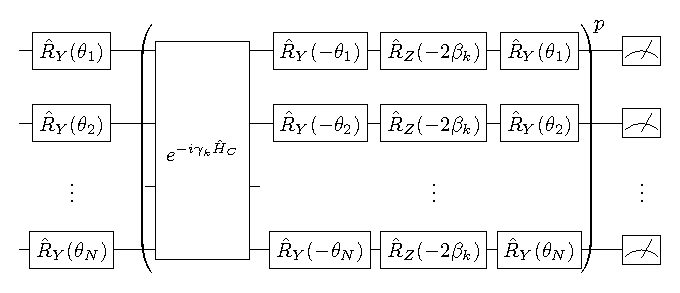
\includegraphics[height=0.3\textheight]{figures/warmstart/figure02.pdf}\end{center}}
\ona{\begin{figure}[htb]\centering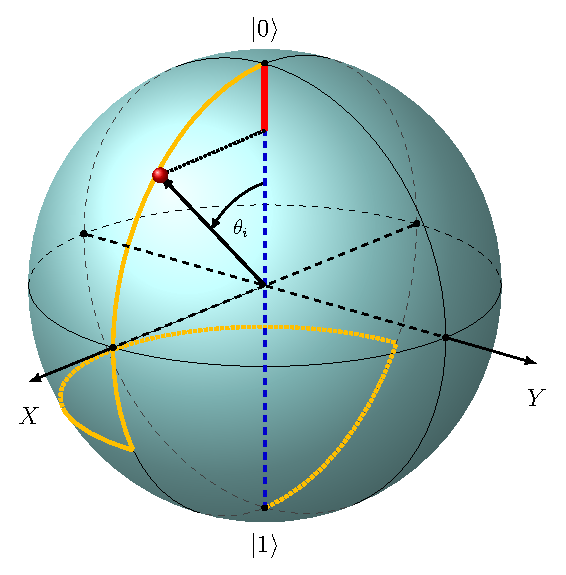
\includegraphics[width=0.42\linewidth]{figures/warmstart/figure01.pdf}\hfill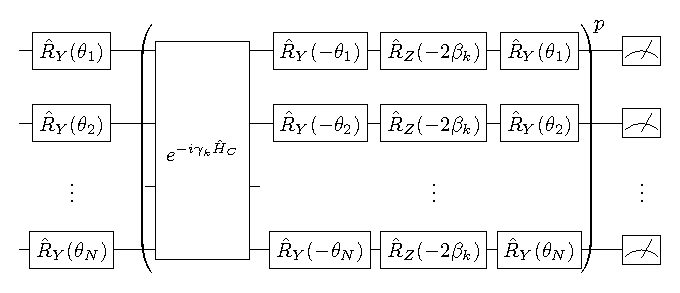
\includegraphics[width=0.5\linewidth]{figures/warmstart/figure02.pdf}\caption{Left: initial state $R_Y(\theta_i)\ket0$ on the Bloch sphere; the dashed line from $\ket0$ to $\ket1$ is the interval $[0,1]$, the red line the relaxed solution $c_i^\star$, and $\varepsilon$ restricts the allowed angles; the orange path is the evolution under the mixer at $c_i^\star = 0$, $\varepsilon = 0.25$, $\beta = \pi/2$. Right: the WS-QAOA circuit \cite{egger2021warm}.}\label{fig:ch11:bloch}\end{figure}}
\ona{\label{fig:ch11:circuit}}
\end{frame}

\begin{frame}\ft{Reachability and the regularisation $\varepsilon$}
\ona{If $c_i^\star \in \{0,1\}$, qubit $i$ starts in $\ket0$ or $\ket1$ and, since $H_C$ contains only $Z_iZ_j$ and identity terms, stays there forever: if the relaxed and the binary optimum disagree on that coordinate, the optimum is unreachable. Hence a regularisation $\varepsilon \in [0,0.5]$:}
\begin{equation}\label{eq:ch11:eps}
    \theta_i = \begin{cases} 2\arcsin\sqrt{c_i^\star} & c_i^\star \in [\varepsilon, 1-\varepsilon],\\ 2\arcsin\sqrt{\varepsilon} & c_i^\star < \varepsilon,\\ 2\arcsin\sqrt{1-\varepsilon} & c_i^\star > 1-\varepsilon,\end{cases}
\end{equation}
\ona{with the mixer adjusted accordingly.}
\begin{itemize}\setlength\itemsep{0.2em}
    \item $\varepsilon$ interpolates continuously between WS-QAOA and standard QAOA: at $\varepsilon = 0.5$ the initial state is $\ket{+}^{\otimes n}$ and the mixer is $-\sum X_i$.
    \item If all $c_i^\star \in (0,1)$ or $\varepsilon > 0$, WS-QAOA converges to the optimum as $p\to\infty$, exactly as standard QAOA: the initial state is the ground state of the mixer and overlaps every basis state, so the adiabatic argument of \Chap~\chref{C.QAOA} applies.
    \item The point of optimising angles is to \emph{beat} the adiabatic schedule at small $p$.
\end{itemize}
\end{frame}

\section{Simulations}

\begin{frame}\ft{Continuous warm start: portfolio optimization}
\ona{The test problem is portfolio selection \cite{Markowitz1952} with a budget: $\min_x q\,x^\top\Sigma x - \mu^\top x$ subject to $\boldsymbol 1^\top x = B$, with $n = 6$ assets, $B = 3$, $q = 2$, the constraint enforced by a penalty $\lambda(\boldsymbol 1^\top x - B)^2$, $\lambda = 3$. Covariances and returns come from simulated price series; $c^\star$ from CPLEX; angles from COBYLA seeded uniformly in $\pm2\pi$; statevector simulation.}
\figslide[height=0.5\textheight]{figures/warmstart/figure04.pdf}{(a) Probability of sampling the optimal portfolio and (b) energy of the optimised state versus depth for standard QAOA, WS-QAOA, and the warm initial state with the standard mixer; medians and quartiles over ten seeds \cite{egger2021warm}.}{fig:ch11:pevo}
\end{frame}

\begin{frame}\ft{Continuous warm start: 250 instances and annealing}
\ona{At depth one on 250 random instances, standard QAOA piles up at $0.74\,E_0$ while WS-QAOA spreads up to $E_0$, with the gain largest when relaxed and binary optima overlap (Fig.~\ref{fig:ch01:depth1} in \Chap~\chref{C.Motivation}). From the annealing viewpoint, Trotterised evolution from the mixer ground state needs less time $T$ and fewer steps $N$ with the warm-start mixer than with the transverse field:}
\figslide[height=0.45\textheight]{figures/warmstart/figure06.pdf}{Normalised energy after Trotterised annealing with the warm-start mixer (a) and the equal-superposition mixer (b), as a function of total time $T$ and number of steps $N$; (c) time-resolved energy at the marked points \cite{egger2021warm}.}{fig:ch11:anneal}
\end{frame}

\section{Comparison and outlook}

\begin{frame}\ft{Rounded versus continuous warm starts}
\begin{center}\ona{\small}\onp{\scriptsize}
\begin{tabular}{lcc}\toprule
 & rounded (\Chap~\chref{C.WSRounded}) & continuous (this \chap) \\\midrule
relaxation & SDP, then random-hyperplane rounding & convex QP over $[0,1]^n$ \\
initial state & a cut, regularised by $\varepsilon$ & product state with $\mathrm{Pr}[x_i=1] = c_i^\star$ \\
mixer & rotated so that $(\pi/2, 0)$ reproduces the cut & rotated so that $\ket{\phi^\star}$ is its ground state \\
guarantee & inherits $\alpha_{\rm GW}$ for any angles & inherits the relaxation's quality at $\boldsymbol\theta = 0$ \\
convergence in $p$ & not covered by the adiabatic argument & adiabatic argument applies \\
needs & $\Sigma$ arbitrary & $\Sigma \succeq 0$ (or a PSD projection) \\
qubits & $n$ & $n$ ($\Theta(n^2)$ to encode $Y^\star$ directly) \\\bottomrule
\end{tabular}
\end{center}
\ona{Both are instances of the design space of \Chap~\chref{C.WSRounded}: what to round, when, and how. The portfolio problem of this \chap{} is developed in full in \Chap~\chref{C.Portfolio}.}
\end{frame}

\begin{frame}\ft{Other warm starts}
\begin{itemize}\setlength\itemsep{0.3em}
    \item Polynomially solvable special cases of QUBO, and low-rank approximations of $\Sigma$ or of the SDP solution.
    \item Time-limited runs of exact solvers (CPLEX, Gurobi): the incumbent is a warm start, as it is in classical branch and bound.
    \item Encoding the matrix-valued SDP solution $Y^\star$ in a $\Theta(n^2)$-qubit state, then a parametrised circuit that contains the identity, then measurement: strong guarantees, too many qubits for now.
    \item In VQE, the particle-hole representation around the Hartree--Fock state is a warm start (\Chap~\chref{C.VQE}); in general, any good classical solution is one.
    \item Warm starts also address barren plateaus: a parametrisation that starts close to the optimum does not start on the plateau.
\end{itemize}
\ona{An implementation of WS-QAOA is available in Qiskit Optimization.}
\end{frame}

\begin{frame}[allowframebreaks]\ft{References}
\biblio
\end{frame}

\end{document}
